\documentclass{article}
\usepackage[margin=1in]{geometry}
\usepackage{amssymb}
\usepackage{etoolbox}
\usepackage{graphicx}
\usepackage{algorithm}
\usepackage{algpseudocode}
\usepackage{float}
\usepackage{etoolbox}
\usepackage{tikz}
\usepackage{dsfont}
\usetikzlibrary{tikzmark}
\usetikzlibrary{calc}

\errorcontextlines\maxdimen

% begin vertical rule patch for algorithmicx (http://tex.stackexchange.com/questions/144840/vertical-loop-block-lines-in-algorithmicx-with-noend-option)
% note that some of the packages above are also needed
\newcommand{\ALGtikzmarkcolor}{black}% customise this, if you want
\newcommand{\ALGtikzmarkextraindent}{4pt}% customise this, if you want
\newcommand{\ALGtikzmarkverticaloffsetstart}{-.5ex}% customise this, if you want
\newcommand{\ALGtikzmarkverticaloffsetend}{-.5ex}% customise this, if you want
\makeatletter
\newcounter{ALG@tikzmark@tempcnta}

\newcommand\ALG@tikzmark@start{%
	\global\let\ALG@tikzmark@last\ALG@tikzmark@starttext%
	\expandafter\edef\csname ALG@tikzmark@\theALG@nested\endcsname{\theALG@tikzmark@tempcnta}%
	\tikzmark{ALG@tikzmark@start@\csname ALG@tikzmark@\theALG@nested\endcsname}%
	\addtocounter{ALG@tikzmark@tempcnta}{1}%
}

\def\ALG@tikzmark@starttext{start}
\newcommand\ALG@tikzmark@end{%
	\ifx\ALG@tikzmark@last\ALG@tikzmark@starttext
	% ignore this, the block was opened then closed directly without any other blocks in between (so just a \State basically)
	% don't draw a vertical line here
	\else
	\tikzmark{ALG@tikzmark@end@\csname ALG@tikzmark@\theALG@nested\endcsname}%
	\tikz[overlay,remember picture] \draw[\ALGtikzmarkcolor] let \p{S}=($(pic cs:ALG@tikzmark@start@\csname ALG@tikzmark@\theALG@nested\endcsname)+(\ALGtikzmarkextraindent,\ALGtikzmarkverticaloffsetstart)$), \p{E}=($(pic cs:ALG@tikzmark@end@\csname ALG@tikzmark@\theALG@nested\endcsname)+(\ALGtikzmarkextraindent,\ALGtikzmarkverticaloffsetend)$) in (\x{S},\y{S})--(\x{S},\y{E});%
	\fi
	\gdef\ALG@tikzmark@last{end}%
}



% the following line injects our new tikzmarking code
\apptocmd{\ALG@beginblock}{\ALG@tikzmark@start}{}{\errmessage{failed to patch}}
\pretocmd{\ALG@endblock}{\ALG@tikzmark@end}{}{\errmessage{failed to patch}}
\makeatother
% end vertical rule patch for algorithmicx

\patchcmd{\thebibliography}{\section*{\refname}}{}{}{}
\usepackage{url}
\renewenvironment{abstract}
{\small
	\begin{center}
		\bfseries \abstractname\vspace{-.4em}
	\end{center}
	\list{}{
		\setlength{\leftmargin}{2cm}
		\setlength{\rightmargin}{\leftmargin}
	}
	\item\relax}
{\endlist}
\date{}
\begin{document}
	\begin{center}
		\large{\rule{420pt}{0.4pt}}\\
		\vspace{0.15in}
		\LARGE{\bfseries{Attention-Over-Actions Option-Critic}}
		\vspace{0.1in}
		\large{\rule{420pt}{0.4pt}}
		
		\large{Computer Science Extended Essay}
		
		\normalsize{Word Count: about 2971}
	\end{center}
	\vspace{0.1in}
	\section*{Research Question}
	How can localized options be trained in the Option-Critic architecture? \\
	\vspace{0.1in}
	\begin{abstract}
	Option discovery in Reinforcement Learning has become quite popular recently. Since the proposal of Option-Critic, many follow up papers has focused on improving it, many of which ended up with a set of diverse and localized options. In this essay, I will propose a framework for algorithms to produce localized options, then base on the framework, I will derive a new algorithm that categorize sub-task based on the use of actions. This algorithm will be called Attention-Over-Actions Option-Critic because the action vector is Hadamard multiply with an attention mechanism.
	\end{abstract}
	\section{Introduction}
	\qquad \ As human we operate in high level actions. For example when driving a car, we make decisions about turning left or right instead of thinking about which muscle to contract. We human have the ability to temporally abstract a chain of actions into one single high level action. 
	
	\quad In Reinforcement Learning, we have a way to capture this idea of temporally abstract action by using options \cite{SUTTON1999181}. When options are defined, learning the policy-over-options are very straight forward, by using SMDP Q-Learning \cite{smdp} or Intra-Option Learning \cite{intraoplearn}. However, if the options are not given and need to be learned, things get a lot harder since it requires knowing what makes an option good. 

	\quad Many people argue that a good options should be diverse and localized \cite{khetarpal2020options}. One of the recent papers \cite{attentionoptioncritic} follows this assumption by requiring options to attend to different features of the state. This essay focus on extending this idea of abstraction from state to action. 
	
	\quad This essay will be structured as follows: First, preliminary and related work will be presented to give a context to what I am trying to do. Second, previous work will be analyzed to figure out why they work. Third, a framework will be proposed based on the observations made in the analysis. Forth, an algorithm will be derived from the framework. Finally, the algorithm will be evaluated in Four Room and the Mujoco environment \cite{mujoco}.
	\section{Preliminary}
	\qquad \ This section only acts as a summary. You are assumed to have basic knowledge about Hierarchical Reinforcement Learning.
	\subsection*{Markov Decision Process}
	\qquad \  Markov decision process (MDP) \cite{sutton2018reinforcement} is a mathematical framework for modeling decision making in a stochastic environment. It is defined as a tuple: $<\mathcal{S}, \mathcal{A}, r, \gamma, P>$ where:
	
	$\mathcal{S}$ is the set of states.
	
	$\mathcal{A}$ is the set of actions
	
	$r : \mathcal{S} \times \mathcal{A} \rightarrow \mathbb{R}$ is the reward function
	
	$\gamma \in [0,1)$ is the discount factor that ensure the cumulative reward $\sum_{t=0}^{\infty} \gamma^t r(s_t, a_t)$ converges
	
	$P : \mathcal{S} \times A \times \mathcal{S} \rightarrow [0,1]$ is the transition model which gives the probability for a particular transition to occur.
	
	\quad All MDPs are said to have the Markov Property, which means that $P(s,a,s')$ only depends on the current state and action. In an MDP, A policy $\pi : \mathcal{S} \times \mathcal{A} \rightarrow [0,1]$ is responsible for choosing the action, after an action is chosen, the environment transitions to a new state according to $P(s,a,s')$, also a reward is given to the policy, and the cycle continues until the policy arrives a termination state.
	\subsection*{Reinforcement Learning}
	\qquad \ Reinforcement Learning (RL) \cite{sutton2018reinforcement} is a machine learning paradigm which allows an agent to learn from interaction in an MDP. The agent's goal is to maximizes long term return $\sum_{t=0}^{\infty} \gamma^t r(s_t, a_t)$.
	
	\quad Actor-Critic \cite{Konda00actor-criticalgorithms} is one of the popular classes of algorithms that harvest the advantage of both Q-Learning and Policy Gradient. A critic network is trained to minimize the one step TD error $r + \gamma \max_{a'} Q(s',a') - Q(s,a)$, while an actor network simultaneously takes gradient step $Q(s,a) \nabla \log\pi(a|s) $. 
	\subsection*{Option Framework}
	\qquad \ Options \cite{SUTTON1999181} are temporally extended actions. They are defined as a tuple: $<\mathcal{I}_\omega,\pi_\omega,\beta_\omega>$, where:
	
	\qquad $\mathcal{I}_\omega \subseteq \mathcal{S}$ is the initiation set that define which state the option can be selected
	
	\qquad $\pi_\omega : \mathcal{S} \times \mathcal{A} \rightarrow [0,1]$ is the internal policy
	
	\qquad $\beta_\omega:\mathcal{S} \rightarrow [0,1]$ is the termination probability.
	
	\quad In an MDP, a policy-over-options $\pi_\Omega : \mathcal{S} \times \Omega \rightarrow [0,1]$, where $\Omega$ is the set of options, selects one of the options to execute, then actions are chosen by the current option's $\pi_\omega$ from then on, until the option terminated according to its $\beta_\omega$, then $\pi_\Omega$ selects an option again. An option has a chance to terminate after an action is executed. Options can be viewed as a generalization for actions, since an option can become an action by setting $\mathcal{I}_\omega=\mathcal{S}$, $\pi_\omega(a|s)=1$ and $\beta_\omega(s)=1$ everywhere.
	
	\quad The policy-over-options $\pi_\Omega$ can be derived by first training $Q_\Omega$ using SMDP Q-Learning \cite{smdp} $Q(s,\omega)\leftarrow Q(s,\omega) + \alpha(r + \gamma^k \max_{\omega'} Q(\omega',\omega') - Q(s,\omega))$ or Intra-Option Learning \cite{intraoplearn} $Q(s,\omega)\leftarrow Q(s,\omega) + \alpha(r + \gamma ((1-\beta(s'))Q(s',\omega)+\beta(s')\max_{\omega'}Q(s',\omega')) - Q(s,\omega))$, then make the $\pi_\Omega$ greedy policy of $Q_\Omega$.
	\section{Related Work}
	\qquad \ In this section, some of the other option discovery algorithms will be summarized.
	\subsection*{Option-Critic}
	\qquad \ Option-Critic \cite{bacon2016optioncritic} is an RL algorithm inspired by Action-Critic \cite{Konda00actor-criticalgorithms}. termination functions $\beta_\omega$ and option-policies $\pi_\omega$ takes gradient steps to maximize expected return, while a option-value function $Q_\Omega$ take gradient steps to minimize error between itself and the empirical return.
	\subsection*{Deliberation Cost}
	\qquad \ Since optimal policy can be achieved even without using options, if options are trained only to maximize expected return, the options may slowly degenerate, which means they either terminate every steps or dominate. Deliberation Cost \cite{harb2017waiting} is a way to encourage longer option duration by punishing the option for every termination.
	\subsection*{Interest Option-Critic}
	\qquad \ The original Option-Critic assumes that options can be initiated everywhere, Interest Option-Critic \cite{khetarpal2020options} tries to remove this assumption by introducing interest functions $I:\mathcal{S} \times \Omega \rightarrow [0,1]$ as an approximation for the initiation set. Experimental results show that options learned by Interest Option-Critic is localized.
	\subsection*{Termination-Critic}
	\qquad \ While other work in this section focus on improving Option-Critic by adding features to the algorithm, Termination-Critic \cite{harutyunyan2019termination} aims to change the objective of the termination function $\beta$. Instead of maximizing the expected return, $\beta$ is trained to minimize the entropy of the termination state. In other words, making the termination state more predictable.
	\subsection*{Attention Option-Critic}
	\qquad \ Attention Option-Critic \cite{attentionoptioncritic} implements attention mechanism into Option-Critic. Different options are trained to attend to different features of the state. The attention units were trained to not only maximize the expected return, but also other things like maximizing difference between attention of different options.
	\section{Exploration}
	\qquad \ An analysis on localization will be conducted in this section.
	\subsection*{What is Localization?}
	\qquad \ Localization is about options each responsible for a sub-task, or another way of looking at it is options each representing a skill. For example in environments like Four Rooms or T-maze, each localized options will be used in a small area of the 2D space. However, in environments where agent can move further in the state space per step, such as visual inputs, each localized options will be used in states that are near temporally. One of the signs for localization is having long options duration. However, defining and measuring localization quantitatively is hard, which is why most work evaluate these option discovery algorithms qualitatively, by observing the agent acting for an episode in the environment.
	\subsection*{Why Localization?}
	\qquad \ To understand why we want localization, first we need to answer a fundamental question: Why do we even use options in the first place? Is it to maximize expected return? However, optimal policy can be achieved using only primitive actions. If options cannot give us a higher return, why do we even need options? Some researchers suggest that options should speed up planning \cite{harb2017waiting} \cite{harutyunyan2019termination} and also options should be transferable \cite{khetarpal2020options} \cite{attentionoptioncritic}. If this is what a good option should be like, then a set of localized options would be beneficial. Localized options are more interpretable, which makes it easily reusable when transferred to a different environment. Also, interpretable options can speed up planning because each options have its clear purpose and usage.
	\subsection*{How Localization is achieved?}
	\qquad \ Now I will analyze how some of the previous work achieve localization of options.\vspace{0.15in}\\
	\large{\bfseries{Attention Option-Critic}}\vspace{0.05in}
	
	\normalsize{\quad In Attention Option-Critic \cite{attentionoptioncritic}, each options are trained to attend to different features of the state. My hypothesis is that the attention mechanism can act as a constraint on what kind of policy each option can have. Each features of the state represents a piece of information about the state. When performing a sub-task, not all the features are necessary. Each sub-task requires different subset of features. Since the attention mechanism limits the subset of features given to an option, the option cannot learn sub-task that requires features outside of the subset of features it was given, or else the option will perform poorly. In the algorithm, each option is trained to have diverse attention, which force each option to learn to complete a different sub-task. For example, there is 3 options and an RGB 2D image is the features of the state. Suppose the 3 options each attend to one of the RGB channels, and one of the sub-tasks is checking if there is a red circle on the image. In this case, only the option with attention on the red channel can complete this sub-task.}\vspace{0.15in}\\
	\large{\bfseries{Deliberation Cost}}\vspace{0.05in}
	
	\normalsize{\quad In Deliberation Cost \cite{harb2017waiting}, options are encouraged to be more temporally extended. My hypothesis is that the algorithm does not directly make options more localized, it instead eliminates all options that are not localized for sure. Since options that terminate every steps are not localized for sure, adding a Deliberation Cost can eliminates all of these options, which makes training localized options more probable.}\vspace{0.15in}\\
	\large{\bfseries{Termination-Critic}}\vspace{0.05in}
	
	\normalsize{\quad In Termination-Critic \cite{harutyunyan2019termination}, option termination states' entropy is being minimized, and experimental results show that option trained by this usually choose to terminate in bottleneck states (frequently visited states). My hypothesis is that bottleneck states are usually the start or end of a sub-task, having the option terminate at these states essentially chains termination with initiation. I will illustrate this with a simple example: In the Four Rooms environment, assume that the sub-task is walking from one doorway to another. The two doorway are bottleneck states because the agent must go through them. Since the agent can take on many paths, all the other states are not bottleneck states. When the agent get to the next doorway, another option can be immediately initiated.}
	\begin{figure}[h]
		\centering
		\large{(a)}
		
\includegraphics[width=1.5in]{termCrit1.png}
		\hspace{0.2in}
		\large{(b)}
		
\includegraphics[width=1.5in]{termCrit2.png}
		\hspace{0.2in}
		\large{(c)}
		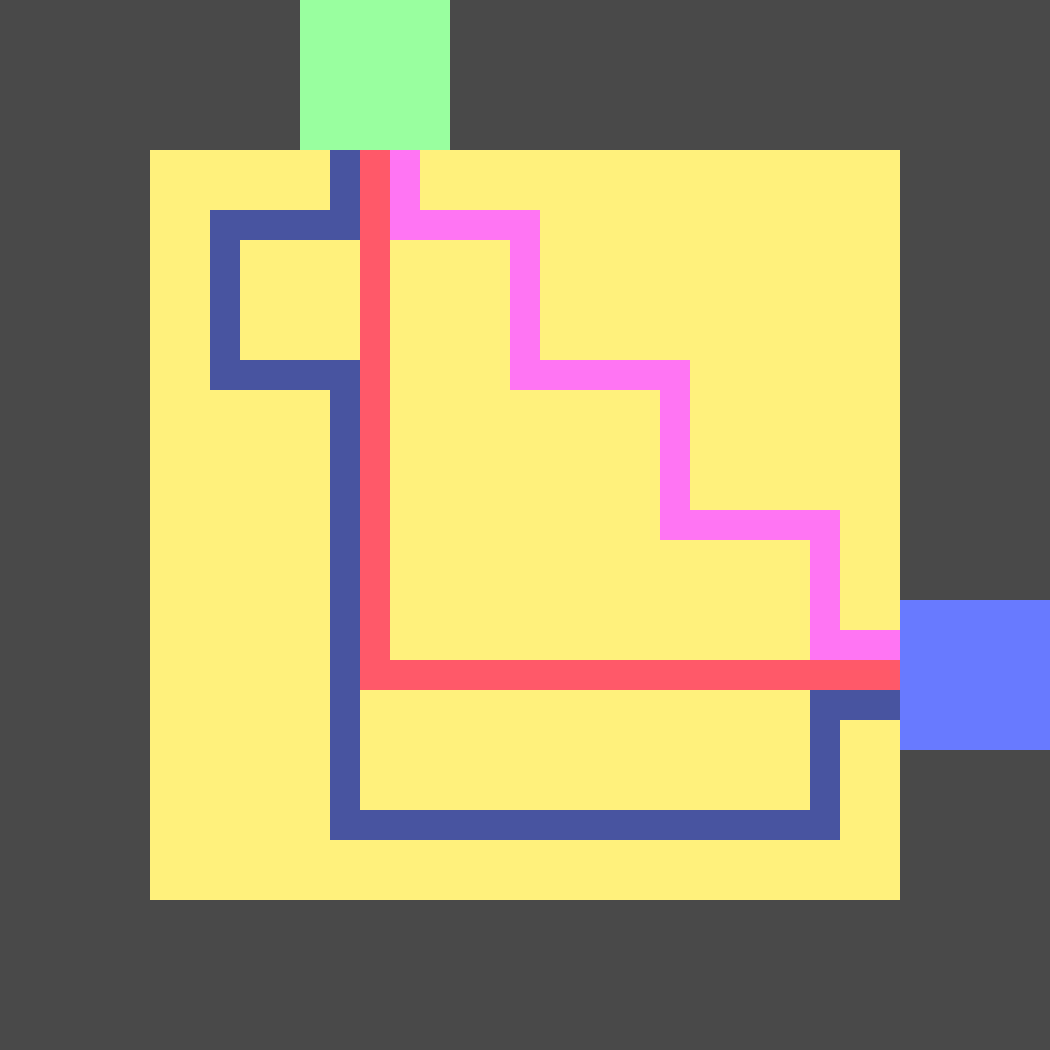
\includegraphics[width=1.5in]{termCrit3.png}
		\caption{(a) and (b) are two options in the theoretic example. Green is the start of the option, blue is the end of the option, yellow is the intermediate states. (c) is a zoomed-in version of the bottom left room. Dark blue, red and pink lines are some of the paths the option can take.}
	\end{figure}\vspace{0.15in}\\
	\large{\bfseries{Interest Option-Critic}}\vspace{0.05in}

	\normalsize{\quad To me Interest Option-Critic just seems like magic. Firstly, it is trained to maximize total return only, but it still achieved localization. Secondly, in the code, the policy-over-options is also trained with gradient ascent, which makes the policy-over-options the same as the interest function, except that one is softmax and one is sigmoid. My best guess is that the interest function provides an easier way to learn localized options. The combination of sigmoid and softmax function is easier to achieve localization than just a softmax function. And according to the experimental results in the original paper, Interest Option-Critic actually perform slightly better than Option Critic, which means that there is a chance that localized option can have a higher return. So Interest Option-Critic can and have the motivation to achieve localized option while Option-Critic may stuck in local maximum.}
	\section{The Localization Framework}
	\qquad \ Naturally, the next question that will be asked is: What do all of these algorithms have in common? Now I will propose a frame work that can act as an abstraction for all of these algorithms.\vspace{0.1in}\\
	\rule{420pt}{2pt}\vspace{0.1in}\\
	\large{\bfseries{The Localization Framework}}\\
	\rule{420pt}{0.4pt}\\
	\normalsize{\bfseries{1. Categorization}}
	
	\normalsize{Divide the whole task into meaningful sub-tasks based on a certain criterion}\\
	{\bfseries{2. Assignment}}
	
	\normalsize{Assign the divided sub-tasks to different options}\\
	{\bfseries{3. Optimization}}
	
	\normalsize{Train options to perform well in the sub-task it is given and also improve the initial categorization of sub-tasks}\\
	{\bfseries{4. Selection}}
	
	\normalsize{Form the policy-over-options to select option in different situation}\\
	\rule{420pt}{1pt}\vspace{0.1in}
	
	\quad This framework is inspired by Adaboost \cite{adaboost}, which is an Ensemble Learning algorithm from Supervised Learning. There are a lot of similarities between Ensemble Learning and Option Learning, this has already been pointed out in previous work \cite{zhang2018ace}, the individual weak classifiers can be thought of as options, each weak classifier is responsible for classifying a small subset of the training data, just like how each option is responsible for a sub-task. In Adaboost, a bunch of weak classifiers are trained sequentially, each of them focuses on training data that is classified poorly by the previous weak classifiers. Since this training process can be seen as dividing training example into category, then assign it to different weak classifiers, it inspires the Categorization and Assignment steps in the Localization Framework. Also, the Optimization step in the framework is reminiscent of the weak classifiers learning to classify the training examples. After a lot of weak classifiers are trained, Adaboost combines them together to form a boosted classifier. The boosted classifier is the weighted sum of all the weak classifiers, the weighting is somewhat like a selection process, so it inspires the Selection step in the framework.
	\begin{table}[H]
		\begin{center}
			\begin{tabular}{|p{23mm}||p{30mm}|p{30mm}|p{30mm}|p{30mm}|}
				\hline
				&&&&\\
				&\centering \bfseries Categorization&\centering \bfseries Assignment&\centering \bfseries Optimization&\bfseries \hspace{0.25in} Selection \\
				\hline\hline
				&&&&\\
				\bfseries Deliberation Cost&\small Divide states based on their temporal closeness&\small The deliberation cost is put on the termination function of each option&\small Option minimize deliberation cost and maximize return, the temporal categorization is very vague and can be changed easily &\small Choose the option with maximum expected return including deliberation cost\\
				&&&&\\
				\hline
				&&&&\\
				\bfseries Attention Option-Critic&\small Divide sub-tasks based on the features they need from state&\small The algorithm assign an attention mechanism to each option&\small Option maximize return, the attention mechanism maximize return and also difference between attention&\small Choose the option with maximum expected return\\
				&&&&\\
				\hline
				&&&&\\
				\bfseries Termination-Critic&\small Divide sub-task based on bottleneck states&\small The termination functions are trained to terminate in bottleneck states&\small Internal policy maximize return, termination function minimize entropy&\small Choose the option with maximum expected return\\
				&&&&\\
				\hline
			\end{tabular}
			\caption{All previous algorithms can be fitted into the Localization Framework, except for Interest Option-Critic because I still couldn't really figure out why it works}
		\end{center}
	\end{table}
	\quad All of the previous algorithms can be seen as an implementation of this framework. This framework is the abstraction of algorithms that produce localized options, so it is very useful in deriving a new algorithm in the next section.
	\section{Attention-Over-Actions Option-Critic}
	\qquad \ Now that there is a framework, I can just follow the framework and derive a new algorithm. The following algorithm will be called Attention-Over-Actions Option-Critic because it perform abstraction on the action space, this algorithm is largely inspired by Attention Option-Critic.
	\begin{figure}[h]
		\centering
		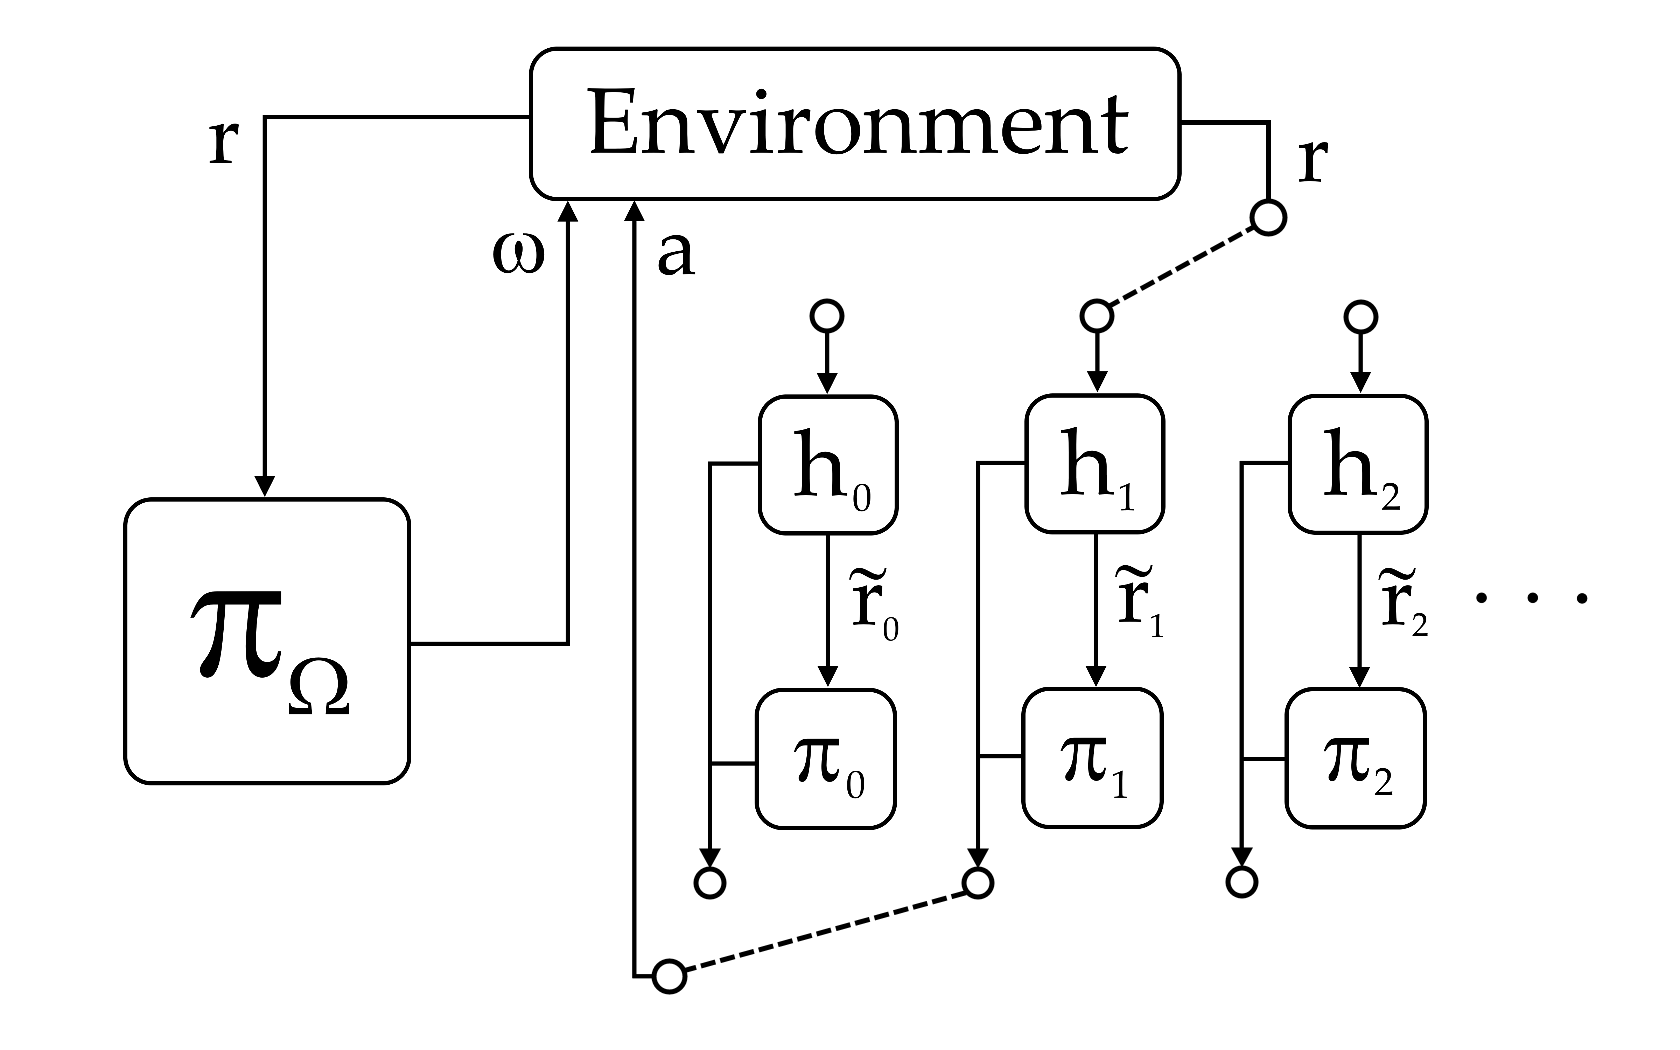
\includegraphics[width=4in]{aoaoc.png}
		\caption{Visualization of the interaction between the environment and the Attention-Over-Actions Option-Critic algorithm. Note that the state is ignored here for clearer presentation.}
	\end{figure}
	\subsection*{1. Categorization}
	\qquad \ In Attention Option-Critic, the Categorization step divide sub-tasks based on features needed, this works because each sub-task requires a different subset of features. The following algorithm borrow the idea of attention over state features and apply it to actions, so each option will attend to different sets of actions. The intuition for this is that each sub-task will not need to use all the actions, for example, when you are watching a film, you will not need to move your hands. This is essentially performing actions abstraction, since the option can attend to a subset of the actions.
	\subsection*{2. Assignment}
	\qquad \ The following algorithm assigns the sub-task in a similar way as Attention Option-Critic, an attention mechanism $h_{\omega,\phi}:\mathcal{A} \rightarrow [0,1]$ parameterized by $\phi$ will be given to each option. But instead of masking the state features, it masks the probability for choosing each actions. So the final probability $\pi_{h_\omega}$ for option $\omega$ to choose action $a$ will be: $$\pi_{h_\omega}(a|s) = \frac{\pi_{\omega,\theta}(a|s)h_{\omega, \phi}(a)}{\sum_{a'} \pi_{\omega,\theta}(a'|s)h_{\omega, \phi}(a')}$$ \qquad \ where $\pi_{\omega,\theta}$ is the internal policy of option $\omega$ and is parameterized by $\theta$.
	
	\quad $\pi_{h_\omega}$ can also be expressed in matrix form: $$\pi_{h_\omega}(s) = \frac{\pi_{\omega,\theta}(s)\odot h_{\omega, \phi}}{\pi_{\omega,\theta}(s)^\intercal h_{\omega, \phi}}$$ \qquad \ Where all of these are column matrix with each component corresponding to one action, and $\odot$ is the Hadamard product.
	\subsection*{3. Optimization}
	\qquad \ Optimization is probably the step that requires the most decision made when designing this algorithm, but luckily optimization of the attention mechanism and that of the option can designed separately.\vspace{0.2in}\\
	{\bfseries Option Optimization}\vspace{0.05in}
	
	\quad Let's first consider the optimization of the option. Normally, when optimizing the internal policy, we will perform gradient ascent on the return: $$\theta \leftarrow \theta + \alpha_\theta \nabla_\theta Q_\Omega(s,\omega)$$ \qquad \ where $Q_\Omega(s,\omega)$ is the expected return for choosing $\omega$ in $s$
	
	\quad I can now directly reuse the result from the Option-Critic paper, and only change $\pi_{\omega,\theta}$ to $\pi_{h_\omega}$: $$\nabla_\theta Q_\Omega(s,\omega) = E[\nabla_\theta \pi_{h_\omega}(a|s) Q_\omega(s,\omega,a)]$$
	\qquad \ However, this is not desirable because the behavior of the optimal policy would not change, any policy can be achieved by simply dividing the attention mechanism and then normalize: $$\widetilde{\pi}_{\omega,\theta}(a|s) = \frac{\pi_{\omega,\theta}(a|s) }{h_{\omega, \phi}(a)\sum_{a'} (\pi_{\omega,\theta}(a'|s)/h_{\omega, \phi}(a'))}$$
	
	\quad What I really want is for the option to accept the attention mechanism, instead of fighting against it. I want the option to find the next best action provided that there is a constraint. So a better way to optimize the internal policy is to devalue the Q-value of the unattended actions, this way the option will not know that it can actually cheat the system by dividing the attention mechanism. One way to devalue the Q-value is to punish the policy for choosing an action that the option is not attending to. Just like Deliberation Cost, the reward $r$ is transformed into a pseudo-reward $\widetilde{r}_\omega$: $$\widetilde{r}_\omega(s,a)=r(s,a)-\rho_\omega(a)$$ \qquad \ It seems to me that the choice of the punishment $\rho_\omega$ can be arbitrary, as long as it is large when $h_{\omega,\phi}$ is small. So I will just choose it like this:$$\rho_\omega(a)=\xi R (1-h_{\omega,\phi}(a)^n)$$ $$\textrm{where } R=\max_{s,a}r(s,a)-\min_{s,a}r(s,a)$$ $$ \textrm{and } n\geq 1\geq\xi>0$$
	
	\quad There is some intuition behind this definition. $n$ is for making sure that all actions with low attention will be treated almost the same, while actions with high attention will be treated differently even for a small difference. $R$ is an attempt to scale the punishment with the reward, so if all the rewards are suddenly doubled, the punishment will still have the same effect. $\xi$ can be interpreted as an exploratory constant, because this value scales the punishment, which can also be interpreted as the motivation to try actions that it is not attending to. This punishment $
	\rho$ will be called the Distraction because it is high when the option chooses actions it is not attending to.
	
	\quad Now we can learn expected return after choosing an action $\widetilde{Q}_U$ and expected return after choosing an option $\widetilde{Q}_\Omega$ to approximate the expected pseudo-return using Q-Learning. After we have the Q-values, we can train $\pi_{\omega,\theta}$ and $\beta{\omega, \nu}$ just like in the original Option-Critic.\vspace{0.2in}\\
	{\bfseries Attention Mechanism Optimization}\vspace{0.05in}
	
	\quad Now let's consider the optimization of $h_{\omega,\phi}$. I want the categorization to be different for all options because or else all options will just aim for the sub-task with highest return. I also want the options to focus on as little actions as possible while still having acceptable performance. Essentially what I need is the algorithm to consider the trade-off between these objectives and achieve a balance between them. A nice way to do this is to add all of these objective up and then perform gradient ascent on the sum: $$\phi \leftarrow \phi + \alpha_\phi \nabla_\phi \sum_{o} (w_o O_o)$$ \qquad \ where $o$ is the index of an objective, $w_o$ is the weight of the objective, $O_o$ is the objective function.
	\quad This method has been used for Attention Option-Critic too. Now I will list out the objectives that I want the option to consider: 
	
	\qquad 1. Perform well
	
	\qquad 2. Different from other options
	
	\qquad 3. The components of the attention mechanism is close to 0 or 1
	
	\qquad 4. Focus on small set of actions
	
	\quad For the first objective, I can just use $Q_\Omega(s,\omega)$ like in Attention Critic. Note that this objective uses the real Q-value instead of the pseudo-Q-value. $$O_1=\max_h Q_\Omega(s,\omega)$$
	
	\quad For the second objective, I will minimize cosine similarity just like in Attention Critic. Cosine similarity is desirable because magnitude doesn't matter, only the angle does. A small change in a short vector will correspond to a large change in the angle. While small change in a long vector will not change the angle much. Which means that the cosine similarity is more sensitive to large similar components. This is what we want because when we are comparing two attention mechanism, we only do not want both to have high attention on the same action, we don't care if both have low attention on the same action.$$O_2 = \min_h \sum_{h' \neq h} \frac{<h', h>}{||h'||+||h||}$$
	
	\quad For the third objective, I will minimize entropy in the attention mechanism. Entropy measures the uncertainty in a probability distribution, so $h$ must be normalized first. This actually also slightly optimize the forth objective since only attending to 1 actions have the lowest uncertainty.$$O_3 = \max_h <\frac{h}{||h||},\log \frac{h}{||h||}> \textnormal{ where log is elementwise}$$
	
	\quad For the forth objective, I will minimize the Minkowski distance of the attention mechanism. This is similar to minimizing the length of the attention mechanism, which discourage focusing on too many actions. Having $p<1$ is for making small values more prominent, which slightly optimize the third objective.$$O_4 = \min_h ||h|| \textnormal{ where }||.||\textnormal{ is Minkowski distance with } p<1$$
	
	\subsection*{4. Selection}
	\qquad \ Any policy-over-options that favor higher Q-value options will work in this case, because the option will need the right set of actions in order to perform well, or else it will fail horribly. So the Q-value already encoded which option has the right set of actions. This means that policies like $\epsilon$-Greedy should work for this algorithm.
	
	\subsection*{Intuition for this algorithm}
	\qquad \ Option Framework is very similar to a construction site, options are the workers and actions are the tools(e.g. Hammer or Shovel). In this algorithm, each option pay attention to only a small set of actions and learn a policy that use them well. This can be drawn parallel with workers only focusing on learning a few tools and master them. Each worker will be responsible for a sub-task in a construction project, in other words, there will be division of labour. 
	
	\quad In this algorithm, the components in the attention mechanism are not binary and can take on any real numbers between 0 and 1. In the context of construction site, there are two interpretation for a non-integer focus on a tool. First it can be interpreted as the worker not trying hard enough when learning the tool. Interestingly, this interpretation is parallel to the first method suggested in the Optimization section: $\theta \leftarrow \theta + \alpha_\theta \nabla_\theta Q_\Omega(s,\omega)$. The worker have the incentive to learn a good tool even if he is not focusing on it, just like how the option have the incentive to use a good action even if it is not attending to it. The second interpretation is that the worker is given a weaker tool, this interpretation is parallel to the punishment method suggested in the Optimization section: $\widetilde{r}_\omega(s,a)=r(s,a)-\rho_\omega(a)$. The workers will not have the incentive to learn a tool that they are not focusing on, even if the normal version of the tool can bring a higher wage, because the worker is only given a weaker version of the tool.
	
	\quad One of the objectives that the attention mechanism need to optimize is the global Q-value $Q_\Omega(s,\omega)$, while the option's internal policy optimizes a local Q-value $\widetilde{Q}_\Omega(s, \omega)$. This can be drawn parallel with the manager in a construction project, since the manager usually see things from a broader perspective.\vspace{0.1in}
	
	\begin{algorithm}[H]
	\caption{Pseudocode for Attention-Over-Actions Option-Critic (AOAOC)}
	\begin{algorithmic}
		\vspace{1.5mm}
		\State $s \leftarrow s_0$
		\State Choose $\omega$ according to the policy-over-options $\pi_\Omega(s)$
		\Repeat
		\State Choose $a$ according to $\pi_{h_\omega}(a|s)$
		\State Take action $a$ in $s$, observe $s'$, $r$\vspace{3mm}
		\State \bfseries{1. Options evaluation:}
		\State $\widetilde{r}_\omega\leftarrow r-\rho_\omega(a)$
		\State \normalfont $\widetilde{\delta} \leftarrow \widetilde{r}_\omega - \widetilde{Q}_U(s,\omega,a)$
		\State \normalfont $\delta \leftarrow r - Q_U(s,\omega,a)$
		\If{$s'$ is non-terminal}
		\State $\widetilde{\delta} \leftarrow \widetilde{\delta}+\gamma(1-\beta_\omega(s'))\widetilde{Q}_\Omega(s',\omega)+\gamma \beta_\omega(s')\max_{\omega'}\widetilde{Q}_\Omega(s',\omega')$
		\State $\delta \leftarrow \delta+\gamma(1-\beta_\omega(s'))Q_\Omega(s',\omega)+\gamma \beta_\omega(s')\max_{\omega'}Q_\Omega(s',\omega')$
		\EndIf
		\State $\widetilde{Q}_U(s,\omega,a)\leftarrow \widetilde{Q}_U(s,\omega,a) + \widetilde{\alpha} \widetilde{\delta}$
		\State $Q_U(s,\omega,a)\leftarrow Q_U(s,\omega,a) + \alpha \delta$
		\vspace{3mm}
		\State {\bfseries1. Options improvement:}
		\State $\theta \leftarrow \theta + \alpha_\theta \nabla_\theta \log \pi_{h_\omega}(a|s)\widetilde{Q}_U(s,\omega,a)$
		\State $\nu \leftarrow \nu + \alpha_\nu \nabla_\nu \beta_{\omega,\nu}(s')(\widetilde{Q}_\Omega(s',\omega)-\widetilde{V}_\Omega(s')$
		\State \normalfont $\phi \leftarrow \phi + \alpha_\phi \nabla_\phi \sum_{o} (w_o O_o)$
		\If{$\beta_{\omega,\nu}$ terminates in $s'$}
		\State {choose new $\omega$ according to the policy-over-options $\pi_\Omega(s)$}
		\EndIf
		\State $s \leftarrow s'$
		\Until $s'$ is terminal
		
	\end{algorithmic}
	\end{algorithm}
	\section{Evaluation}
	\section{Conclusion}
	\section{Future Direction}
	\qquad \ This algorithm currently only focuses on discrete action space, a possible future direction might be extending this to continuous space. For vector actions, it might be good to attend to only some of the components of the vector, while ignoring other components by either randomly selecting values for them or keeping them the same as in the last state of the previous option. For scalar action, one direction is to use a one dimensional gaussian distribution as the attention mechanism, and multiply it with the original action distribution. However, some sort of trick may need to be deployed to speed up the process of normalization.
	\section{Bibliography}
	\bibliographystyle{ieeetr}
	\bibliography{bibliography}
	\section{Appendix}
	\subsection*{Notations}
	{\bfseries Markov Decision Process}\\
	$\mathcal{S}$ --- Set of states\\
	$\mathcal{A}$ --- Set of actions\\
	$r$ --- Reward function or reward\\
	$\gamma$ --- Discount factor\\
	$P$ --- Transition model\\
	$\pi$ --- Policy\\
	$s$ --- State\\
	$a$ --- Action\\
	$s_T$ --- Termination state\\
	{\bfseries Option Framework}\\
	$\Omega$ --- Set of options\\
	$\pi_{\omega,\theta}$ --- Internal policy of option $\omega$\\
	$\beta_\omega$ --- Termination probability of option $\omega$\\
	$\mathcal{I}_\omega$ --- Initiation set of option $\omega$\\
	$\pi_\Omega$ --- Policy-over-options\\
	$Q_U$ --- Expected return for choosing an action\\
	$Q_\Omega$ --- Expected return for choosing an option\\
	$\theta$ --- Parameter for internal policy\\
	$\nu$ --- Parameter for termination probability\\
	$\omega$ --- option\\
	{\bfseries Attention-Over-Actions Option-Critic}\\
	$h_{\omega,\phi}$ --- Attention Mechanism\\
	$\pi_{h_\omega}$ --- Final probability\\
	$\phi$ --- Parameter for attention mechanism\\
	$\rho$ --- Distraction\\
	$R$ --- Difference between max and min reward\\
	$n$ --- Power constant in $\rho$\\
	$\xi$ --- Exploratory constant in $\rho$\\
	$\widetilde{r}$ --- Pseudo-reward\\
	$\widetilde{Q}_U$ --- Expected pseudo-return from choosing an action\\
	$\widetilde{Q}_\Omega$ --- Expected pseudo-return from choosing an option\\
	$\widetilde{V}_\Omega$ --- Expected pseudo-return for being in a state\\
	$\widetilde{\alpha}$ --- Learning rate for $\widetilde{Q}_U$\\
	$\alpha$ --- Learning rate for $Q_U$\\
	$\alpha_\theta$ --- Learning rate for internal policy\\
	$\alpha_\nu$ --- Learning rate for termination probability\\
	$\alpha_\phi$ --- Learning rate for attention mechanism\\
	$R$ --- Minimum reward clipped by 0\\
	$O_o$ --- Objective function\\
	$w_o$ --- Weight of objective function\\
	$o$ --- Objective\\
	$\delta$ --- One step Q-value error\\
	$\widetilde{\delta}$ --- One step pseudo-Q-value error\\
	{\bfseries Operations}\\
	$\odot$ --- Hadamard product (elementwise product)\\
	$\nabla$ --- Gradient\\
	$^\intercal$ --- Matrix transpose\\
	$E[\ ]$ --- Expected value\\
	$\leftarrow$ --- Assignment\\
	$<,>$ --- Dot product\\
	$||.||$ --- Norm of a vector unless specify\\
	\subsection*{Proof}
	\subsection*{Experimental Details}
	\subsection*{Code}

\end{document}